\chapter{Special relativity}
\section{The principle of relativity}
First, we assume there is an upper limit of velocity of propagation of interaction $c$. Second, we assume that inertial reference frame are all the same in describing the law of physics. Then, we can find the invariant intervals when transforming from one inertial reference frame to another, $ds^2 = -c^2 dt^2 + dx^2 + dy^2 + dz^2$. 
(In the following, we adopt the unit system in which $c$ equals $1$.) The transformation between different inertial frame preserving the intervals is called Lorentz transformation, which can be written as
\[\overline{x}^{\mu} = \Lambda^{\mu}_{\phantom{\mu}\nu} x^{\nu}\]
The invariant symbol of the vector representation of Lorentz transformation is $\eta^{\mu \nu}$
\[\Lambda^{\mu}_{\phantom{\mu}\rho}  \Lambda^{\nu}_{\phantom{\nu}\sigma}  \eta^{\rho \sigma} = \eta^{\mu \nu},\]
where,
\[\eta^{\mu \nu} \equiv \left[ 
\begin{matrix} 
-1& & & \\ 
& +1 & & \\
& & +1 & \\
& & & +1
\end{matrix} 
\right]\]
The inverse matrix of $\eta^{\mu \nu}$ is
\[\eta_{\mu \nu} = \left[ 
\begin{matrix} 
-1& & & \\ 
& +1 & & \\
& & +1 & \\
& & & +1
\end{matrix} 
\right]\]
We can use $\eta^{\mu \nu}$ and and its inverse $\eta_{\mu \nu}$ to raise and lower vector indices, 
\[x_{\mu} \equiv \eta_{\mu \nu} x^{\nu}\]
And we can verify the following identities,
\[\Lambda^{\mu}_{\phantom{\rho}\rho} \Lambda_{\nu}^{\phantom{\rho}\rho} = \delta^{\mu}_{\nu} \]
\[x^{\mu} = \eta^{\mu \nu} x_{\nu}\]
\[\overline{x}_{\mu} = \Lambda_{\mu}^{\phantom{\mu}\nu} x_{\nu}\]
\[\Lambda_{\mu}^{\phantom{\mu}\rho}  \Lambda_{\nu}^{\phantom{\nu}\sigma}  \eta_{\rho \sigma} = \eta_{\mu \nu},\]
In a special case where the new reference frame move along $\hat{1}$ direction with velocity $\beta$, we have
\[\overline{x}^{0} = \gamma x^0 - \gamma \beta x^1\]
\[\overline{x}^{1} = -\gamma \beta x^0 + \gamma x^1\]
where $\gamma \equiv (1-\beta^2)^{-1/2}$.
\\ \\
Some physical quantity will behave like a tensor (vector,scalar) when transforming form one inertial frame to another. For example,
\paragraph{scalar} proper time: $d \tau$, mass: $m$, electrical charge $e$
\paragraph{vector} four velocity: $u^{\mu} \equiv \frac{dx^{\mu}}{d \tau}$, four momentum: $p^{\mu} \equiv m u^{\mu}$, four acceleration: $a^{\mu} \equiv \frac{du^{\mu}}{d \tau}$, four force: $f^{\mu} \equiv m a^{\mu}$.\\ \\
We can also define the corresponding three vector.
\paragraph{three velocity}: $\hat{v}^{i} \equiv \frac{dx^i}{dt}$
\[u^0 = \gamma_v, u^i = \gamma \hat{v}^i\]
If the new reference frame move along $\hat{1}$ direction with velocity $\beta$, we have
\[\overline{\hat{v}}^1 = \frac{\hat{v}^1 - \beta}{1-\hat{v}^1 \beta}\]
\[\overline{\hat{v}}^2 = \frac{\hat{v}^2}{\gamma(1-\hat{v}^2 \beta)}\]
\[\overline{\hat{v}}^3 = \frac{\hat{v}^3}{\gamma(1-\hat{v}^3 \beta)}\]
\paragraph{three momentum}: $\hat{p}^{i} \equiv p^i$
\paragraph{three acceleration}: $\hat{a}^{i} \equiv \frac{dv^i}{dt}$
\paragraph{three force}: $\hat{f}^i \equiv \frac{d\hat{p}^i}{dt}$
\[f^i = \gamma_v \hat{f}^i\]

\section{Relativistic Mechanics}
For a free particle, we have following equations of motion:
\[\frac{dp^{\mu}}{d\tau} = 0\]
It can be formulated in several ways
\subsubsection{Lagrangian formulation}
\[S=-m\int_{a}^{b} d\tau, \ \ \ \ \delta x^{\mu}(a) = \delta x^{\mu}(b) = 0\]
\[\delta S = 0 \Rightarrow m\frac{du^{\mu}}{d\tau} = 0\]
\subsubsection{Hamiltonian formulation}
\[S = \int_{t_1}^{t_2} L dt \quad L = - m \sqrt{1-\dot{x}_i\dot{x}^i}\]
\[\pi^i = \frac{\partial L}{\partial \dot{x}_i} = \gamma m \eta^{ij}\dot{x}_j\]
\[H = \pi^i \dot{x}_i - L = \gamma m = \sqrt{m^2 + \pi^i \pi_i}\]
So, the Hamiltonian equations are
\[\dot{\pi}^i = 0, \ \ \ \ \dot{x_i} = \eta_{ij}\frac{\pi^j}{\sqrt{m^2 + \pi^k \pi_k}}\]
\subsubsection{Hamiltonian-Jacobi equation}
\[H = -\frac{\partial S}{\partial t}, \ \ \ \ \pi^i = \frac{\partial S}{\partial x_i}\]
Note that $p^0 = H$, $p^i = \pi^i$, we have $p^{\mu} = \frac{\partial S}{\partial x_{\mu}}$. So, we can see that $p^{\mu}$ is a vector under Lorentz transformation. The Hamiltonian-Jacobi equation can be written as
\[(\frac{\partial S}{\partial t})^2 = m^2 + (\frac{\partial S}{\partial x})^2 + (\frac{\partial S}{\partial y})^2 + (\frac{\partial S}{\partial z})^2\]
\\ \\
For a non-free particle, we have the revised newton's second law:
\[f^{\mu} = \frac{dp^{\mu}}{d\tau}\]
The formula is the definition of the four force. It can also be written in three vector as
\[\hat{f}^i = \gamma_v m \hat{a}^i + \gamma_v^3 (\hat{a}^j \hat{v}_j) m \hat{v}^i\]
\\ \\
If the system consists of more than one particles interacting with each other. We have the conservation laws from the symmetry.
\subsubsection{Translational symmetry and conservation of momentum}
\[\overline{x}^{\mu} = x^{\mu} + \delta x^{\mu}\]
\[\delta S = \sum p_{\mu} \delta x^{\mu}|_a^b = 0 \]
$\sum p^{\mu}$ is conserved.
\subsubsection{Rotational symmetry and conservation of angular momentum}
\[\overline{x}^{\mu} = x^{\mu} + x_{\nu}\delta \omega^{\mu \nu}\]
where $I+\delta \omega$ is the infinitesimal Lorentz transformation.
\[\delta S = \sum p^{\mu} x^{\nu} \delta \Omega_{\mu \nu}|_a^b = 0 \]
Since $\delta \omega$ is anti symmetric, $\sum M^{\mu \nu} $ is conserved, where $M^{\mu \nu} \equiv x^{\mu}p^{\nu} - x^{\nu}p^{\mu}$.

\section{Relativistic Scattering}
\subsection{Distribution function}
The number of particles in the region $\bm{r}+d\bm{r}$ and $\bm{p} + d\bm{p}$ is $f(\bm{p},\bm{r})dp_x dp_y dp_z dx dy dz$. Then  $f(\bm{p},\bm{r})$ is called distribution function.\\
We first determine the properties of the "volume element" $dp_x dp_y dp_z$, with respect to Lorentz transformations. If we introduce a four-dimensional coordinate system, on whose axes are marked the components of the four-momentum of a particle, then $dp_x dp_y dp_z$, can be considered as the zeroth component of an element of the hypersurface defined by the equation $p^{\mu}p_{\mu} + m^2 = 0$. The element of hypersurface is a four-vector directed along the normal to the hypersurface; in our case the direction of the normal obviously coincides with the direction of the four-vector $p^{\mu}$. From this it follows that the ratio
\[\frac{dp_x dp_y dp_z}{E}\]
is an invariant quantity, since it is the ratio of corresponding components of two parallel four-vectors.\\
Then, we notice that $dVdt$ is invariant under Lorentz transformation and $dt = \frac{E}{m} d\tau $. So we can infer that
\[dx dv dz E\]
is an invariant quantity quantity. Putting all together, we know the phase volume
\[dp_x dp_y dp_z dx dy dz\]
is an invariant volume. So, we have
\[f(\bm{r},\bm{p}) = f'(\bm{r}',\bm{p}')\]
in coordinate transformation.

\subsection{Invariant cross section}
Recall the definition of cross section
\[\sigma \equiv \frac{\mbox{Number of Events per target}}{\mbox{Time} \times \mbox{Incident Flux}}\]
Here, the incident flux and time are measured in the frame of target particle.\\
Suppose that we have two colliding beams; we denote by $n_1$ and $n_2$ the particle densities in them and by $\bm{v}_1$ and $\bm{v_2}$ the velocities of the particles. In the reference system in which particle 2 is at rest, we are dealing with the collision of the beam of particles 1 with a stationary target. Then according to the usual definition of the cross-section $\sigma$, the number of collisions occurring in volume $dV$ in time $dt$ is 
\[dN = \sigma v_{rel} n_1 n_2 dV dt\]
,where $v_{\mathrm{rel}}$ is the velocity of particle 1 in the rest system of particle 2 (which is just the definition of the relative velocity of two particles in relativistic mechanics). \\
The number $dN$ is by its very nature an invariant quantity. We would like to express it in a form which is applicable in any reference system: 
\[dN = A n_1 n_2 dV dt\] 
where $A$ is a number to be determined, for which we know that its value in the rest frame of one of the particles is $v_{\mathrm{rel}} \sigma$. We shall always mean by $\sigma$ precisely the cross-section in the rest frame of one of the particles, i.e. by definition, an invariant quantity. From its definition, the relative velocity $v_{\mathrm{rel}}$ is also invariant. The product dVdt is an invariant. Therefore the product $A n_1 n_2$ must also be an invariant. The law of transformation of the particle density n is
\[n = \frac{n_0}{\sqrt{1-v^2}} = n_0 E/m\]
so we can construct $A$ in an arbitrary frame as
\[A = -\sigma v_{\mathrm{rel}} \frac{p_1^{\mu}p_{2\mu}}{E_1 E_2}\]
Note that
\[-p_1^{\mu}p_{2\mu} = \frac{m_1}{\sqrt{1-v_{\mathrm{rel}}^2}}m_2 = m_1 m_2 \frac{1-\bm{v}_1\cdot\bm{v}_2}{\sqrt{(1-\bm{v}_1^2)\cdot(1-\bm{v}_2^2)}}\]
we can get the following expression for $v_{\mathrm{rel}}$:
\[v_{\mathrm{rel}} = \frac{\sqrt{(\bm{v}_1-\bm{v}_2)^2-(\bm{v}_1\times\bm{v}_2)^2}}{1-\bm{v}_1\cdot\bm{v}_2}\]
Finally, we have
\[dN = \sigma \sqrt{(\bm{v}_1-\bm{v}_2)^2-(\bm{v}_1\times\bm{v}_2)^2} n_1 n_2 dV dt\]
If the velocities $v_1$ and $v_2$ are collinear, then we have
\[dN = \sigma |\bm{v}_1 - \bm{v}_2| n_1 n_2 dV dt\]
If we have only one target, then
\[dN = \sigma |\bm{v}_1 - \bm{v}_2| n_1 dt\]

\subsection{Elastic scattering between two particles}
\[(E_1,\bm{p}_1,E_2,\bm{p}_2) \to (E_1',\bm{p}_1',E_2',\bm{p}_2')\]
In lab frame (L frame),
\[E_2 = m_2 \quad \bm{p}_2 = 0\]
By the conservation of momentum, we can derive that
\[\cos \theta_1 = \frac{E_1'(E_1+m_2)-E_1 m_2 - m_1^2}{p_1 p_1'}\]
\[\cos \theta_2 = \frac{(E_1+m_2)(E_2'-m_2)}{p_1 p_2'}\]
where $\theta_1(\theta_2)$ is the angle between $\bm{p}_1'(\bm{p}_2')$ with $\bm{p}_1$.
In a special case where $m_1 =0$, we have
\[E_1' = \frac{m_2}{1-\cos\theta_1 + \frac{m_2}{E_1}}\]
Let $x \equiv p_1'\cos\theta_1$,$y \equiv p_1'\sin\theta_1$,we can get that
\[\frac{(x-c)^2}{a^2}+\frac{y^2}{b^2}=1\]
where
\[a \equiv \frac{p_1(E_1m_2+m_2^2)}{m_1^2 + m_2^2 + 2m_2 E_1} = \frac{m_2V}{\sqrt{1-V^2}} \quad b \equiv \frac{m_2 p_1}{\sqrt{m_1^2 + m_2^2 + 2m_2 E_1}} = \frac{a}{\sqrt{1-V^2}} \quad c \equiv \frac{ p_1(E_1m_2+m_1^2)}{m_1^2 + m_2^2 + 2m_2 E_1}\]
where $V \equiv \frac{p_1}{E_1 + m_2}$ is the velocity of particle 2 before scattering in C frame. 
And it is easy to see that $a + c = p_1$. 
The result above can be represented by a picture.
\begin{figure}[!h]
	\centering
	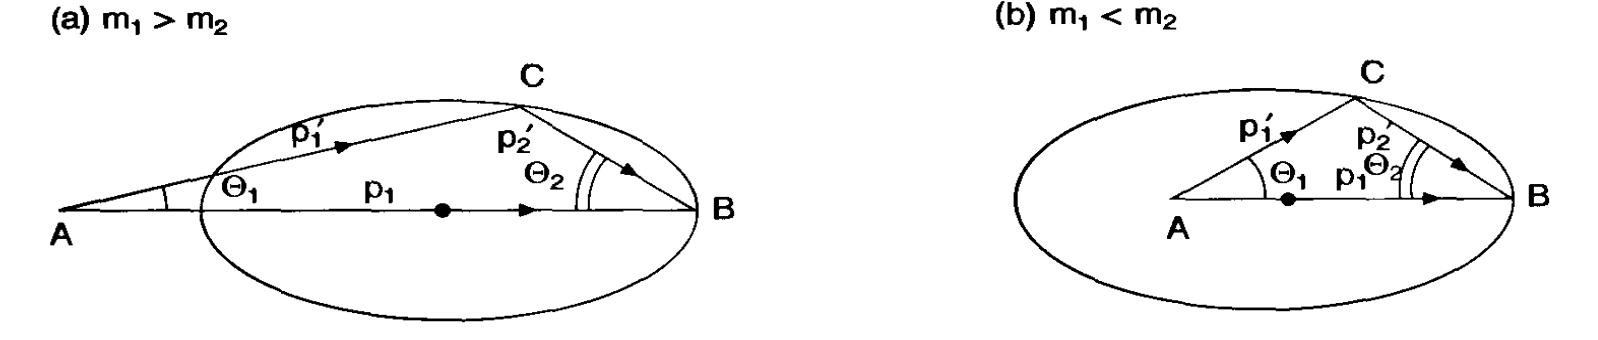
\includegraphics[height=3.4cm ,width=15.98cm]{CFT/scattering.png}
	\caption{Relativistic scattering}
\end{figure}
\noindent
Next, suppose in the center of mass frame (C frame), the scattering angle is $\chi$,then we can derive that
\[E_1' = E_1 - \Delta E \quad E_2' = m_2 + \Delta E\]
where
\[\Delta E \equiv \frac{m_2(E_1^2-m_1^2)}{m_1^2 + m_2^2 + 2m_2E_1}(1-\cos\chi)\]

\chapter{Classical field theory}
\section{Lagrangian formulation}
\[S = \int \mathcal{L}(\phi_a,\dot{\phi}_a,\nabla \phi_a) d^4 x, \ \ \ \ \delta \phi_a |_{\Sigma} = 0\]
\[\delta S = 0 \Rightarrow \partial_{\mu} \left (\frac{\partial \mathcal{L}}{\partial (\partial_{\mu} \phi_a)} \right ) - \frac{\partial \mathcal{L}}{\partial \phi_a} = 0\]
\subsubsection{Locality of the theory}
There are no terms in the Lagrangian coupling $\phi(\bm{x},t)$ directly to  $\phi(\bm{y},t)$ with $\bm{x} \neq \bm{y}$. The closet we get for the $\bm{x}$ label is coupling between $\phi(\bm{x},t)$ and $\phi(\bm{x}+\delta\bm{x},t)$ through the gradient term $\bm{\nabla} \phi$.
\subsubsection{Lorentz invariance}

Scalar fields:
\[\overline{\phi}(x) = \phi(\Lambda^{-1} x)\]
Vector fields:
\[\overline{A}^{\mu}(x) = \Lambda^{\mu}_{\phantom{\mu}\nu} A^{\nu}(\Lambda^{-1}x)\]
\[\overline{A}_{\mu}(x) = (\Lambda^{-1})^{\nu}_{\phantom{\mu}\mu} A_{\nu}(\Lambda^{-1}x) = \Lambda_{\mu}^{\phantom{\mu}\nu}A_{\nu}(\Lambda^{-1}x)\]
\[\overline{\partial_{\mu}\phi}(x) = (\Lambda^{-1})^{\nu}_{\phantom{\mu}\mu} \partial_{\nu} \phi (\Lambda^{-1}x) = \Lambda_{\mu}^{\phantom{\mu}\nu} \partial_{\nu} \phi (\Lambda^{-1}x)\]
Lagrangian must be a scalar, or more loosely, action must be invariant under Lorentz transformation.

\section{Symmetry and conservation law}
\begin{newthem}[Noether's theorem]
	Every continuous symmetry of the Lagrangian gives rise to a conserved current $j^{\mu}(x)$ such that the equation of motion imply $\partial_{\mu} j^{\mu} = 0$.
	Suppose that the infinitesimal transformation is
	\[\phi_a \rightarrow \phi_a + \delta \phi_a\]
	\[\mathcal{L} \rightarrow  \mathcal{L} + \delta \mathcal{L} \]
	and if $\delta \mathcal{L} = \partial_{\mu} K^{\mu}$, we can get
	\[j^{\mu} = -\frac{\partial \mathcal{L}}{\partial (\partial_{\mu} \phi_a)} \delta \phi_a + K^{\mu}\]
\end{newthem}

\subsubsection{space-time translation}
$\overline{x} = x - a$ 
\[j^{\mu} = a_{\nu} T^{\mu \nu}\]
\[T^{\mu \nu} \equiv -\frac{\partial \mathcal{L}}{\partial(\partial_{\mu}\phi_a)} \partial^{\nu} \phi_a + \eta^{\mu \nu} \mathcal{L}\]
If we define $P^{\mu} \equiv \int T^{0 \mu} d^3 x$,then we have the law of momentum conservation:
\[\frac{d P^{\mu}}{dt} = 0\]

\subsubsection{Lorentz Transformation}
$\overline{x}^{\mu} = x^{\mu} + \delta \omega^{\mu}_{\phantom{\mu}\nu} x^{\nu}$\\
The infinitesimal Lorentz transformation can be written as $I+\delta \omega^{\mu}_{\phantom{\mu}\nu}$
\[\delta \omega^{\mu}_{\phantom{\mu}\nu} = \left[ 
\begin{matrix} 
0       & \beta_1   & \beta_2   & \beta_3   \\ 
\beta_1 & 0         & -\theta_3 & \theta_2  \\
\beta_2 & \theta_3  & 0         & -\theta_1 \\
\beta_3 & -\theta_2 & \theta_1  & 0
\end{matrix} 
\right]\]
We assume that
\[\overline{\phi}_a(x) = \mathcal{S}_{a}^{\phantom{a}b}\phi_b(\Lambda^{-1}x)\]
In the limit of infinitesimal Lorentz transformation, we have
\[\mathcal{S}_{a}^{\phantom{a}b} = \delta_{a}^{\phantom{a}b}+\frac{1}{2} \delta \omega_{\alpha \beta} (\Sigma^{\alpha \beta})_{a}^{\phantom{a}b} \]
So, we have
\[j^{\mu} = \frac{1}{2} M^{\mu \nu \rho}  \delta \omega_{\nu \rho}\]
\[M^{\mu \nu \rho} \equiv x^{\nu}T^{\mu \rho} - x^{\rho} T^{\mu \nu} - \frac{\partial \mathcal{L}}{\partial (\partial_{\mu}\phi_a)}(\Sigma^{\nu \rho})_{a}^{\phantom{a}b}\phi_b\]
If we define $M^{\nu \rho} \equiv \int M^{0 \nu \rho} d^3 x$, then we have the law of angular momentum conservation:
\[\frac{dM^{\nu \rho}}{dt} = 0\]

\section{Functional derivatives}
\begin{newdef}[Functional derivatives]
	Given a manifold $M$ representing (continuous/smooth) functions $\rho$ (with certain boundary conditions etc.), and a functional $F$ defined as
	\[F\colon M\rightarrow \mathbb {R} \quad {\mbox{or}}\quad F\colon M\rightarrow \mathbb {C} \,,\]
	the functional derivative of $F[\rho]$, denoted $\frac{\delta F}{\delta \rho}$,is defined by
	\[{\begin{aligned}\int {\frac {\delta F}{\delta \rho }}(x)\phi (x)\;dx&=\lim _{\varepsilon \to 0}{\frac {F[\rho +\varepsilon \phi ]-F[\rho ]}{\varepsilon }}\\&=\left[{\frac {d}{d\epsilon }}F[\rho +\epsilon \phi ]\right]_{\epsilon =0},\end{aligned}}\]
	where $\phi$ is an arbitrary function. The quantity $\epsilon \phi$ is called the variation of $\rho$. 
\end{newdef}
\noindent
Like the derivative of a function, the functional derivative satisfies the following properties, where $F[\rho]$ and $G[\rho]$ are functionals:\\
Linearity:
\[{\frac {\delta (\lambda F+\mu G)[\rho ]}{\delta \rho (x)}}=\lambda {\frac {\delta F[\rho ]}{\delta \rho (x)}}+\mu {\frac {\delta G[\rho ]}{\delta \rho (x)}},\]
where $\lambda$, $\mu$ are constants.\\
Product rule:
\[{\frac {\delta (FG)[\rho ]}{\delta \rho (x)}}={\frac {\delta F[\rho ]}{\delta \rho (x)}}G[\rho ]+F[\rho ]{\frac {\delta G[\rho ]}{\delta \rho (x)}}\,,\]
Chain rules:\\
If $F$ is a functional and $G$ an operator, then
\[{\displaystyle \displaystyle {\frac {\delta F[G[\rho ]]}{\delta \rho }(y)}=\int dx{\frac {\delta F[G[\rho]]}{\delta G[\rho]}}(x)\cdot {\frac {\delta G[\rho ]}{\delta \rho}(x,y)}\ }\]
If $G$ is an ordinary differentiable function $g$, then this reduces to
\[{\displaystyle \displaystyle {\frac {\delta F[g(\rho )]}{\delta \rho}(y)}={\frac {\delta F[g(\rho )]}{\delta g[\rho ]}(y)}\ {\frac {dg(\rho )}{d\rho }(y)}\ } \]
\begin{newprop}[Properties of functional derivatives]
	\[\frac{\delta F}{\delta \rho} (y) = \lim_{\epsilon \to \infty} \frac{1}{\epsilon} \{ F[\rho(x) + \epsilon \delta(x-y)] - F[\rho(x)] \}\]
	\[\frac{\delta f(x)}{\delta f(y)} = \delta(x-y)\]
	\[\frac{\delta}{\delta f(y)} \int g\left( f(x)\right) dx =  g'(f(y))\]
	\[\frac{\delta f'(x)}{\delta f(y)} = \frac{d}{dx}\delta(x-y)\]
	\[\frac{\delta}{\delta f(y)} \int g\left( f'(x)\right) dx = -\frac{d}{dy} g'(f'(y))\]
\end{newprop}

\section{Hamiltonian formulation}
\[\pi^a(x) = \frac{\partial \mathcal{L}}{\partial \dot{\phi_a}}\]
\[\mathcal{H}(\phi_a,\nabla \phi_a,\pi^a) = \pi^a \dot{\phi_a} - \mathcal{L}\]
\[H = \int \mathcal{H} d^3 x\]
Now, we can get the Hamilton equation form $\delta S =0$,
\[\dot{\phi_a}(\bm{x},t) = \frac{\delta}{\delta \pi^a(\bm{x},t)} H = \frac{\partial \mathcal{H}}{\partial \pi^a}\]
\[\dot{\pi^a}(\bm{x},t) = -\frac{\delta}{\delta \phi_a(\bm{x},t)} H = - \frac{\partial \mathcal{H}}{\partial \phi_a} + \left(\frac{\partial \mathcal{H}}{\partial \phi_{a,b}}\right)_{,b}\]

\subsection{Poisson bracket}

First, we define that
\[[\phi_a(\bm{x}),\phi_b(\bm{y})] \equiv [\pi^a(\bm{x}),\pi^b(\bm{y})] \equiv 0\]
\[[\phi_a(\bm{x}),\pi^b(\bm{y})] \equiv \delta^{b}_{a} \delta(\bm{x}-\bm{y})\]
then, we demand that the bracket operation has the same properties as the Poisson bracket in classical mechanics. And we also demand that
\[[\partial_x A(\bm{x}),B(\bm{y})] = \partial_x [A(\bm{x}),B(\bm{y})]\]
and
\[\left[\int d^3 x A(\bm{x}),B(\bm{y})\right] = \int d^3 x [A(\bm{x}),B(\bm{y})]\]
As a result, we can verify that
\[[W[\phi(\bm{x}),\pi(\bm{x})],Z[\phi(\bm{x}),\pi(\bm{x})]] = \int d^3x \left\{ \frac{\delta W}{\delta \phi(\bm{x})} \frac{\delta Z}{\delta \pi(\bm{x})} - \frac{\delta W}{\delta \pi(\bm{x})} \frac{\delta Z}{\delta \phi(\bm{x})} \right\}\]
Especially,
\[[\phi_a(\bm{x}),H] = \frac{\delta }{\delta \pi^a(\bm{x})} H, \ \ \ \ [\pi^a(\bm{x}),H] = -\frac{\delta }{\delta \phi_a(\bm{x})} H\]
So, the Hamilton equation can be written as
\[\dot{\phi_a} = [\phi_a,H], \ \ \ \ \dot{\pi^a} = [\pi^a,H]\]
Further more, we can prove that
\[\frac{dO(\phi,\pi,t)}{dt} = [O,H] + \frac{\partial O}{\partial t}\]
and
\[\frac{d[A,B]}{dt} = [A,\frac{dB}{dt}] + [\frac{dA}{dt},B]  \]

\subsection{Momentum}

It is easy to verify that
\[P^{0} = H, \ \ \ \ P^{i} = \int -\pi^a \partial^i \phi_a d^3 x\]
And we can get the Poisson bracket
\begin{eqnarray}
	\left[\phi_a,P^{\mu}\right] &=& -\partial^{\mu} \phi_a \nonumber \\
	\left[\pi^a,P^{\mu}\right] &=& -\partial^{\mu} \pi^a \nonumber \\
	\left[P^{\mu},P^{\nu}\right] &=& 0 \nonumber 
\end{eqnarray}


\subsection{Angular momentum}

It is easy to verify that
\[M^{\mu \nu} = \int (x^{\mu}T^{0\nu}-x^{\nu}T^{0\mu}-\pi^a(\Sigma^{\mu \nu})_{a}^{\phantom{a}b}\phi_b) d^3 x\]
We define that
\[M_{L}^{\mu \nu} \equiv \int (x^{\mu}T^{0\nu}-x^{\nu}T^{0\mu}) d^3 x \quad M_S^{\mu \nu} \equiv \int (-\pi^a(\Sigma^{\mu \nu})_{a}^{\phantom{a}b}\phi_b) d^3 x\]
\[(L^{\mu \nu})_a^{\phantom{a}b} \equiv -(x^{\mu}\partial^{\nu}-x^{\nu}\partial^{\mu})\delta_a^{\phantom{a}b} \quad (S^{\mu \nu})_a^{\phantom{a}b} \equiv -(\Sigma^{\mu \nu})_a^{\phantom{a}b}\]
So, we can get the Poisson bracket
\[[\phi_a,M_L^{\mu \nu}] = (L^{\mu \nu})_a^{\phantom{a}b} \phi_b \quad [\phi_a,M_S^{\mu \nu}] = (S^{\mu \nu})_a^{\phantom{a}b} \phi_b\]
\[[\pi^a,M_L^{\mu \nu}] = (L^{\mu \nu})_b^{\phantom{b}a}\pi^{b}  \quad [\pi^a,M_S^{\mu \nu}] = - (S^{\mu \nu})_b^{\phantom{b}a} \pi^b \]
Because $\frac{d M^{\mu \nu}}{dt} = 0$, $M^{\mu \nu}$ can commutate with $\frac{d}{dt}$, so
\[[[\phi(x),M^{\mu \nu}],M^{\rho \sigma}] = (L^{\mu \nu}+S^{\mu \nu})(L^{\rho \sigma}+S^{\rho \sigma})\phi(x)\]
At last, we can get the Poisson bracket 
\[[\phi(x),[M^{\mu \nu},M^{\rho \sigma}]] = (L^{\mu \nu}L^{\rho \sigma}-L^{\rho \sigma}L^{\mu \nu} + S^{\mu \nu}S^{\rho \sigma}-S^{\rho \sigma}S^{\mu \nu})\phi(x)\]
Since we can prove that
\[L^{\mu \nu}L^{\rho \sigma}-L^{\rho \sigma}L^{\mu \nu} = -\eta^{\nu \rho}L^{\mu \sigma} + \eta^{\sigma \mu}L^{\rho \nu} + \eta^{\mu \rho}L^{\nu \sigma} - \eta^{\sigma \nu}L^{\rho \mu}\]
if we demand that
\[S^{\mu \nu}S^{\rho \sigma}-S^{\rho \sigma}S^{\mu \nu} = -\eta^{\nu \rho}S^{\mu \sigma} + \eta^{\sigma \mu}S^{\rho \nu} + \eta^{\mu \rho}S^{\nu \sigma} - \eta^{\sigma \nu}S^{\rho \mu}\]
we will get get the Poisson bracket of the $M^{\mu \nu}$,
\[[M^{\mu \nu},M^{\rho \sigma}] = -\eta^{\nu \rho}M^{\mu \sigma} + \eta^{\sigma \mu}M^{\rho \nu} + \eta^{\mu \rho}M^{\nu \sigma} - \eta^{\sigma \nu}M^{\rho \mu}\]
up to the possibility of a term on the right-hand side that commutes with $\phi(x)$ and its derivatives.\\ \\
We now define $J_i \equiv \frac{1}{2} \epsilon_{ijk} M^{jk}$ and $K_i \equiv M^{i0}$, so we have
\[M^{\mu \nu} = \left[ 
\begin{matrix} 
0   & -K_1 & -K_2 & -K_3 \\ 
K_1 & 0    & J_3  & -J_2 \\
K_2 & -J_3 & 0    &  J_1 \\
K_3 & J_2  & -J_1 &  0
\end{matrix} 
\right] \quad \left( 
\delta \omega_{\mu\nu} = \left[
\begin{matrix} 
0       & -\beta_1   & -\beta_2   & -\beta_3   \\ 
\beta_1 & 0         & -\theta_3 & \theta_2  \\
\beta_2 & \theta_3  & 0         & -\theta_1 \\
\beta_3 & -\theta_2 & \theta_1  & 0
\end{matrix} 
\right] \right)\] 
the Poisson bracket can be written as
\begin{eqnarray}
	\left[J_i,J_j\right] &=& \epsilon_{ijk}J_k \nonumber \\
	\left[J_i,K_j\right] &=& \epsilon_{ijk}K_k \nonumber \\
	\left[K_i,K_j\right] &=& -\epsilon_{ijk}J_k \nonumber
\end{eqnarray}
We can use the similar method to derive that
\[[P^{\mu},M^{\rho \sigma}] = \eta^{\mu \sigma}P^{\mu} - \eta^{\mu \rho}P^{\sigma}\]
It can also be written as
\begin{eqnarray}
	\left[J_i,H\right] &=& 0 \nonumber \\
	\left[J_i,P_j\right] &=& \epsilon_{ijk}P_k \nonumber \\
	\left[K_i,H\right] &=& P_i \nonumber \\
	\left[K_i,P_j\right] &=& \delta_{ij}H \nonumber
\end{eqnarray}
At last, we define $L_i \equiv \frac{1}{2} \epsilon_{ijk} M_L^{jk}$ and $S_i \equiv \frac{1}{2} \epsilon_{ijk} M_S^{jk}$
we can demonstrate that
\begin{eqnarray}
	\left[L_i,S_j\right] &=& 0 \nonumber \\
	\left[S_i,P_j\right] &=& 0 \nonumber \\
	\left[L_i,P_j\right] &=& \epsilon_{ijk}P_k \nonumber
\end{eqnarray}

\chapter{Classical Electrodynamics}
\section{The formulation of classical electrodynamics}
\subsection{Maxwell equations and Lorentz force}
The Lagrangian of the EM field $A^{\mu}$ when coupling with current is
\[\mathcal{L} = -\frac{1}{4}F^{\mu\nu}F_{\mu\nu} + j^{\mu} A_{\mu}\]
where
\[F_{\mu\nu} \equiv \partial_{\mu}A_{\nu} - \partial_{\nu}A_{\mu} \quad j^{\mu} \equiv \rho_{\mathrm{e}0} u^{\mu}\]
and $\rho_{\mathrm{e}0}$ is the charge density measured in the frame of charge.
The Euler-Lagrange equation of EM field is
\[\partial_{\nu} F^{\mu\nu} = j^{\mu}\]
The charge conservation equation then follows directly from field equations,
\[\partial_{\mu} j^{\mu} = \partial_{\mu} \partial_{\nu} F^{\mu\nu} = 0\]
For a charged particle moving in EM field with trajectory $x^{\mu}(\tau)$, we have
\[j^{\mu} =  e_a \delta(\bm{r}-\bm{r}_a(t)) \sqrt{1-\bm{v}_a^2} u_a^\mu \]
it follows that
\[\int dV dt j^{\mu} A_{\mu} = \int dx^{\mu} e_a A_{\mu}(x^{\mu}(\tau))\]
so the action for a charged particle when coupling with EM field is
\[S = - m \int d\tau + e\int dx^{\mu} A_{\mu}(x^{\mu}(\tau))\]
We can derive the Euler-Lagrangian equation of the particle:
\[ma_{\mu} = eF_{\mu \nu}u^{\nu}\]
\begin{note}
The Hamiltonian formulation of electrodynamics will be discussed in detail in the Hamiltonian formulation of general relativity and canonical quantization formulation of quantum electrodynamics.
\end{note}
\noindent
We now define the electric field and magnetic field as follows,
\[E^i \equiv F^{0i} = -\dot{A}^i - \nabla^i A^0 \quad B^i \equiv \epsilon_{ijk} \nabla^j A^k\]
We also define $\rho_{\mathrm{e}} \equiv j^0$ and $J^i \equiv j^i$,so
the field equations can then be written as so-called Maxwell equations:
\begin{eqnarray}
	\bm{\nabla} \times  \bm{B} &=& \frac{\partial \bm{E}}{\partial t} +  \bm{J} \nonumber \\
	\bm{\nabla} \times \bm{E} &=& -\frac{\partial \bm{B}}{\partial t} \nonumber \\
	\bm{\nabla} \cdot \bm{E} &=& \rho_{\mathrm{e}} \nonumber \\
	\bm{\nabla} \cdot \bm{B} &=& 0 \nonumber
\end{eqnarray}
The equations of motion of the charged particle can be written as so-called Lorentz force equations:
\[\frac{d\bm{p}}{dt} = e(\bm{E} + \bm{v} \times \bm{B}) \quad \frac{d \mathcal{E}}{dt} = e \bm{E} \cdot \bm{v}\]
\\
We also note that the Field $A$ cannot be completely determined by Maxwell and Lorentz equation. If we make the transformation $A_{\mu} \to A_{\mu} + \partial_{\mu} \xi(x)$, $\mathcal{L}$ and $F^{\mu\nu}$ would be invariant, and the Maxwell and Lorentz equation is still valid. This arbitrariness of $\xi$ is called gauge invariance. The topic will be discussed in detail in QED.

\subsection{Lorentz transformation of fields}
Suppose the new coordinates satisfy that $\overline{x}^{\mu} = \Lambda^{\mu}_{\phantom{\mu}\nu}x^{\nu}$ after Lorentz transformation, then we have
\[\overline{A}^{\mu}(\overline{x}) = \Lambda^{\mu}_{\phantom{\mu}\nu}A^{\nu}(\Lambda^{-1}\overline{x})\]
In a special case where the new reference frame move along $\hat{1}$ direction with velocity $\beta$, we have
\[\overline{x}^{0} = \gamma x^0 - \gamma \beta x^1 \quad \overline{x}^{1} = -\gamma \beta x^0 + \gamma x^1\]
Similarly, for vector potential, we have 
\[\overline{A}^{0} = \gamma A^0 - \gamma \beta A^1 \quad \overline{A}^{1} = -\gamma \beta A^0 + \gamma A^1\]
It can be further written in terms of electric and magnetic field as
\[\overline{E}_1 = E_1 \quad \overline{E}_2 = \gamma E_2 - \gamma \beta B_3 \quad \overline{E}_3 = \gamma E_3 + \gamma \beta B_2\]
\[\overline{B}_1 = B_1 \quad \overline{B}_2 = \gamma B_2 + \gamma \beta E_3 \quad \overline{B}_3 = \gamma B_3 - \gamma \beta E_2\]
or more generally as
\[\bm{\overline{E}} = \gamma(\bm{E}_{\perp} + \bm{\beta} \times \bm{B}) + \bm{E}_{\parallel}\]
\[\bm{\overline{B}} = \gamma(\bm{B}_{\perp} - \bm{\beta} \times \bm{E}) + \bm{B}_{\parallel}\]
If $\beta \ll 1$, we can neglect the higher order of $\beta^2$. So, we have
\[\bm{\overline{E}} = \bm{E} + \bm{\beta} \times \bm{B}\]
\[\bm{\overline{B}} = \bm{B} - \bm{\beta} \times \bm{E}\]
We also note that $F_{\mu\nu}F^{\mu\nu}$ and $\epsilon_{\mu\nu\rho\sigma}F^{\mu\nu}F^{\rho\sigma}$ is invariant under Lorentz transformation. It can be represented by the electric and magnetic field as
\[E^2 - B^2 = \mbox{ inv } \quad \bm{E} \cdot \bm{B} = \mbox{ inv }\]

\subsection{Energy-momentum tensor}
For a free EM field, the energy-momentum tensor is
\[T_{\mathrm{f}}^{\mu \nu} \equiv -\frac{\partial \mathcal{L}}{\partial(\partial_{\mu}A_{\rho})} \partial^{\nu} A_{\rho} + \eta^{\mu \nu} \mathcal{L} = \partial^{\nu}A^{\rho} F^{\mu}_{\phantom{\rho}\rho}-\frac{1}{4}\eta^{\mu\nu}F_{\rho\sigma}F^{\rho\sigma}\]
We note that the energy-momentum tensor defined above is not symmetric, so we define a modified energy-momentum tensor by adding a term $-\partial^{\rho}A^{\nu}F^{\mu}_{\phantom{\rho}\rho}$,i.e.
\[T_{\mathrm{f}'}^{\mu\nu} = F^{\nu\rho}F^{\mu}_{\phantom{\rho}\rho}-\frac{1}{4}\eta^{\mu\nu}F_{\rho\sigma}F^{\rho\sigma}\]
For free EM field, we have $\partial^{\rho}A^{\nu}F^{\mu}_{\phantom{\rho}\rho} = \partial^{\rho}\left(A^{\nu} F^{\mu}_{\phantom{\rho}\rho}\right)$.
So,
\[\partial_{\mu}T_{\mathrm{f}'}^{\mu\nu} = 0 \quad P_{\mathrm{f}'}^{\mu} = P_{\mathrm{f}}^{\mu}\]
From now on, we will use $T_{\mathrm{f}'}$ as the energy-momentum tensor of EM field and omit the prime for simplicity.
The momentum of the free EM field is
\[P_{\mathrm{f}}^{0} = \int dV \frac{1}{2}(\bm{E}^2+\bm{B}^2) \equiv \int dV w \quad P_{\mathrm{f}}^{i} = \int dV \bm{E} \times \bm{B} \equiv \int dV \bm{S}\]
\\ \\
If there also exists charged particles in the system, i.e. the source of EM field, we must also include the energy-momentum tensor of the particles to get the right conservation equation. The energy-momentum tensor of particles is defined as
\[T_{\mathrm{p}}^{\mu\nu} \equiv \sum_a m_a \delta(\bm{r}-\bm{r}_a) \sqrt{1-\bm{v}_a^2} u_a^\mu u_a^{\nu}\]
From this definition, we can get
\[P_{\mathrm{p}}^0 = \sum_a \frac{m_a}{\sqrt{1-\bm{v}_a^2}} \quad \bm{P}_{\mathrm{p}} =  \sum_a \frac{m_a}{\sqrt{1-\bm{v}_a^2}} \bm{v}_a\]
Recall that
\[j^{\mu}_{\mathrm{e}} = \sum_a e_a \delta(\bm{r}-\bm{r}_a) \sqrt{1-\bm{v}_a^2} u_a^\mu \]
We can also define the mass current as
\[j^{\mu}_{\mathrm{m}} \equiv \sum_a m_a \delta(\bm{r}-\bm{r}_a) \sqrt{1-\bm{v}_a^2} u_a^\mu \]
If there is no creation and annihilation of charged particles, and the mass of the particles is constant during the motion, we would have mass conservation equation
\[\partial_{\mu} j^{\mu}_{\mathrm{m}a} = 0\]
Recall the Lorentz force equation $m a_{\mu} = eF_{\mu\nu}u^{\nu}$, it can be rewritten as
\[\rho_{\mathrm{m}0a} \frac{du_{\mu}}{d\tau} = F_{\mu\nu}j_{\mathrm{e}a}^{\nu}\]
where $\rho_{\mathrm{m}0a} \equiv m_a \delta(\bm{r}-\bm{r}_a) \sqrt{1-\bm{v}_a^2}$ is the mass density measured in the rest frame of the particle.
\\
On the one hand, we have
\[\partial_{\mu} T_{\mathrm{p}}^{\mu\nu} = \sum_a \rho_{\mathrm{m}0a}u^{\mu} \frac{\partial u_a^{\nu}}{\partial x^{\mu}} = \sum_a \rho_{\mathrm{m}0a} \frac{d u_a^{\nu}}{d \tau} = F^{\nu}_{\phantom{\nu}\mu}j_{\mathrm{e}}^{\mu}\]
On the other hand, we can derive that
\[\partial_{\mu} T_{\mathrm{f}}^{\mu\nu} = - F^{\nu}_{\phantom{\nu}\mu}j_{\mathrm{e}}^{\mu}\]
by implementing Maxwell equations.
\\
Define
\[T^{\mu \nu} \equiv T_{\mathrm{f}}^{\mu\nu} + T_{\mathrm{p}}^{\mu\nu}\]
We have
\[\partial_{\mu} T^{\mu\nu} = 0\]
We define the Maxwell stress tensor as
\[f^{ij} \equiv -T_{\mathrm{f}}^{ij} = E^{i}E^{j} + B^{i}B^{j} - w\delta^{ij}\]
Then, we can write down the conservation laws of energy and momentum as
\[\frac{d}{dt}\left(P_{\mathrm{p}}^0 + \int w dV \right) = -\oint \bm{S}\cdot d\bm{\sigma}\]
\[\frac{d}{dt}\left(\bm{P}_{\mathrm{p}} + \int \bm{S} dV \right) = \oint \bm{f}\cdot d\bm{\sigma}\]
We assume there is no particle cross the boundary.
\\
At last, because $T^{\mu\nu} = T^{\nu\mu}$, we have
\[\partial_{\mu}(x^{\nu}T^{\mu\rho}-x^{\rho}T^{\mu\nu}) = 0\]
It is easy to write down the conservation law of angular momentum as
\[\frac{d}{dt}\left(\bm{L}_{\mathrm{p}} + \int \bm{r} \times \bm{S} dV \right) = \oint \bm{r} \times \bm{f}\cdot d\bm{\sigma}\]
where
\[\bm{L}_{\mathrm{p}} \equiv \sum_a \frac{m_a}{\sqrt{1-\bm{v}_a^2}} \bm{r}_a  \times \bm{v}_a \]

\subsection{Charged particles in a given EM field}
Now we suppose the EM field is given, i.e. we will neglect the EM field generated by the test charged particles. Then we have
\[S = \int_{t_1}^{t_2} (-\sqrt{1-v^2}m + e\bm{A}\cdot\bm{v}-e\phi)dt\]
So,
\[L = -\sqrt{1-v^2}m + e\bm{A}\cdot\bm{v}-e\phi\]
The canonical momentum is
\[\bm{\pi} = \frac{\partial L}{\partial \bm{v}} = \gamma m \bm{v} + e \bm{A}\]
The Hamiltonian is therefore
\[H = \bm{\pi} \cdot \bm{v} - L = \gamma m + e \phi = \sqrt{m^2+(\bm{\pi}-e\bm{A})^2}+e\phi\]
If $v \ll 1$, we have
\[L = \frac{mv^2}{2} + e\bm{A}\cdot\bm{v}-e\phi \quad \bm{\pi} =  m \bm{v} + e \bm{A} \quad H = \frac{(\bm{\pi}-e\bm{A})^2}{2m}+e\phi\]
If the EM field is constant in time, we have
\[\bm{\nabla} \times \bm{E} = 0\]
and we could choose the gauge that
\[\dot{\bm{A}} = 0 \quad \bm{E} = -\bm{\nabla} \phi\]
Because $\frac{\partial L}{\partial t}=0$, $\gamma m + e\phi$ is a constant.

\subsubsection{Motion in a uniform and constant electric field}
Suppose the direction of electric field is  $\hat{x}$, the orbit is in the $x-y$ plane. So, the equation of motion is
\[\dot{p}_x = eE \quad \dot{p}_y = 0\]
The final solution is
\[x = \frac{1}{eE}\sqrt{\mathcal{E}_0^2 + (eEt)^2} \quad y = \frac{p_0}{eE} \mathrm{arcsinh} \frac{eEt}{\mathcal{E}_0}\]
Here, we assume $p_x = 0$, $p_y=p_0$ at $t = 0$.
The trajectory of the particle is
\[x = \frac{\mathcal{E}_0}{eE}\cosh \frac{eEy}{p_0}\]

\subsubsection{Motion in a uniform and constant magnetic field}
Suppose the direction of magnetic field is $\hat{z}$. Note that particle's kinetic energy $\mathcal{E} = \gamma m$ is constant if there are no electric field, we can derive the equation of motion
\[\dot{v}_x = \omega v_y \quad \dot{v}_y = -\omega v_x \quad \dot{v}_z = 0\]
where $\omega \equiv \frac{eB}{\gamma m}$. The final solution is
\[x = x_0 + r\sin(\omega t + \alpha) \quad y = y_0 + r\cos(\omega t + \alpha) \quad z = z_0 + v_{0z}t\]
where $x_0,y_0,z_0,r,\alpha,v_{0z}$ should be determined by initial condition.

\subsubsection{Motion in a uniform and constant EM field}
We only focus on the case where the velocity of particle is much smaller than the velocity of light. 
Suppose the direction of magnetic field is $\hat{z}$, the direction of electric field is within $y-z$ plane. The equation of motion is
\[m\ddot{x} = eB\dot{y} \quad m\ddot{y} =eE_y - eB\dot{x} \quad m\ddot{z}=eE_z\]
The solution is
\[\dot{x} = a \cos \omega t + \frac{E_y}{B} \quad \dot{y} = -a\sin \omega t \quad \dot{z} = v_{0z} + \frac{eE_z}{m}t\]
where $\omega = \frac{eB}{m}$ , $a,v_{z0}$ is determined by initial condition. As we suppose that $v \ll 1$ is satisfied,we must have that
\[a \ll 1 \quad v_{0z} \ll 1 \quad \frac{eE_z t}{m} \ll 1 \quad \frac{E_y}{B} \ll 1\]

\section{Constant electromagnetic field}
\subsection{Coulomb' law}
For constant electric field, Maxwell equations take the form 
\[\bm{\nabla} \cdot \bm{E} = \rho_{\mathrm{e}} \quad \bm{\nabla} \times \bm{E} = 0\]
So, we have
\[\bm{E} = -\bm{\nabla} \phi \quad \nabla^2 \phi = -\rho_{\mathrm{e}} \]
The solution is
\[\phi(\bm{r}) = \int  \frac{\rho_{\mathrm{e}}(\bm{r}')}{4\pi|\bm{r}-\bm{r}'|} dV'\]
If $\rho_{\mathrm{e}}(\bm{r}') = Q \delta(\bm{r}')$, we have
\[\phi(\bm{r}) =  \frac{Q}{4\pi|\bm{r}|} \quad E(\bm{r}) = \frac{Q\bm{r}}{4\pi|\bm{r}|^3}\]
For a system of static charged particles, the total energy is
\[U = \frac{1}{2}\int E^2 dV = \frac{1}{2} \int \rho \phi dV = \frac{1}{2} \sum e_a \phi_a + \frac{1}{2}\sum e_a \Phi_a\]
Here, $\phi_a$ is the electric potential at the point where $e_a$ is located, produced by $e_a$ itself, while  $\Phi_a$ is the potential produced by other charges. It is obvious that $U_{\mathrm{self}} = \frac{1}{2} e_a \phi_a$ is infinite, indicating that classical electrodynamics is no more valid in small distance. This problem will be solved in quantum electrodynamics: the mass of charged particle we measured is already renormalized to include the electromagnetic self energy. So, actually, we have
\[U = \frac{1}{2}\int E^2 dV - U_{\mathrm{self}} = \frac{1}{2}\sum_{a \ne b} \frac{e_a e_b}{4\pi R_{ab}}\]
If the charged particle is moving with a constant velocity, we can derive the electric field it produced by Lorentz transformation, the final result is that
\[\bm{E} = \frac{e\bm{R}}{4\pi R^3} \frac{1-V^2}{(1-V^2\sin^2\theta)^{3/2}} \quad \bm{B} = \bm{V} \times \bm{E}\]
where $\bm{R}$ is the vector point from the particle to the point we measure the electric field, and $\theta$ is the angle between $\bm{V}$ and $\bm{R}$.If $V \sim 1$, the electric field will be concentrated in the direction perpendicular to the $\bm{V}$. If $\bm{V} \ll 1$, we have
\[\bm{E} = \frac{e\bm{R}}{4\pi R^3} \quad \bm{B} = \frac{e\bm{V} \times\bm{R}}{4\pi R^3}\]

\subsection{Multipole moments}
For a system of charged particles, the potential it produced at $\bm{R}$ is
\[\phi = \sum_a \frac{e_a}{4\pi|\bm{R} - \bm{r}_a|}\]
If $R \gg r_a$, we can expand the equation around $r_a=0$. Generally, we have
\[\frac{1}{|\bm{R} - \bm{r}|} = \sum_{l=0}^{\infty} \sum_{m=-l}^{l} \frac{r^l}{R^{l+1}} \frac{4\pi}{2l+1} Y^*_{lm}(\Theta,\Phi)Y_{lm}(\theta,\phi)\]
So,we have
\[\phi = \sum \phi^{(l)}\]
where
\[\phi^{(l)} \equiv \frac{1}{4\pi R^{l+1}} \sum_{m=-l}^{l} \sqrt{\frac{4\pi}{2l+1}} Q_{m}^{(l)} Y^*_{lm}(\Theta,\Phi)\]
\[Q_m^{(l)} \equiv \sum_a e_a r_a^l \sqrt{\frac{4\pi}{2l+1}} Y_{lm}(\theta_a,\phi_a)\]
Leading terms: 
\[\phi^{(0)} = \frac{Q}{4\pi R} \quad E^{(0)} = \frac{Q\bm{n}}{4\pi R^2} \quad Q = \sum_a e_a\]
\[\phi^{(1)} = \frac{\bm{d} \cdot \bm{n}}{4\pi R^2}  \quad E^{(1)} = \frac{3(\bm{d}\cdot\bm{n})\bm{n}-\bm{d}}{4\pi R^3} \quad \bm{d} = \sum_a e_a \bm{r}_a\]
\[\phi^{(2)} = \frac{\bm{n} \cdot \bm{D} \cdot \bm{n}}{8\pi R^3} \quad E^{(2)} = \frac{5(\bm{n} \cdot \bm{D} \cdot \bm{n})\bm{n} - (\bm{n} \cdot \bm{D} + \bm{D} \cdot \bm{n})}{8\pi R^4} \quad D_{ij} = \sum e(3x_ix_j-r^2\delta_{ij})\]
For a system of charged particles in the electric field $\phi(\bm{r})$, if all the particles is near the $r=0$, we can make the expansion
\[\phi(\bm{r}) = \sum_{l=0}^{\infty} r^l \sum_{m=-l}^{m=l} a_{lm} \sqrt{\frac{4\pi}{2l+1}} Y_{lm}(\theta,\phi)\]
So
\[U = \sum_{l=0}^{\infty} U^{(l)} \quad U^{(l)} = \sum_{m=-l}^{l} a_{lm}Q^{(l)}_m\]
Leading terms: 
\[U^{(0)} = Q\phi_0 \quad F^{(0)} = Q\bm{E}_0\]
\[U^{(1)} = -\bm{d}\cdot \bm{E}_0 \quad F^{(1)} = \bm{d}\cdot \bm{\nabla}\bm{E}_0 \quad M^{(1)} = \bm{d} \times \bm{E}_0\]
\[U^{(2)} = -\frac{1}{6}\bm{D}\cdot \bm{\nabla}\bm{E}_0 \quad F^{(2)} = \frac{1}{6} \bm{D}\cdot \bm{\nabla}\bm{\nabla}\bm{E}_0 \quad M^{(2)} = \frac{1}{3} \bm{\nabla} \cdot (\bm{D} \times \bm{E}_0)\]

\subsection{Biot-Savart law}
Let us consider the magnetic field produced by charges which perform a finite motion, in which the particles are always within a finite region of space and the momenta also always remains finite. Consider the time average magnetic field $\overline{\bm{B}}$ , produced by the charges; this field will now be a function only of the coordinates and not of the time. We take the time average of the Maxwell equations
\[\bm{\nabla} \cdot \bm{B} = 0 \quad \bm{\nabla} \times \bm{B} = \frac{\partial \bm{E}}{\partial t} + \bm{j}\] 
Note that the average value of the derivative $\partial \bm{E} / \partial t$, like the derivative of any quantity which varies over a finite range, is zero. We can get
\[\bm{\nabla} \cdot \overline{\bm{B}} = 0 \quad \bm{\nabla} \times \overline{\bm{B}} =  \overline{\bm{j}}\]
Recall that $\bm{B} = \bm{\nabla} \times \bm{A}$. We impose the gauge condition $\bm{\nabla} \cdot \bm{A} = 0$, we have
\[\nabla^2 \overline{\bm{A}} = - \overline{\bm{j}}\]
The solution is
\[\overline{\bm{A}}(\bm{r}) = \frac{1}{4\pi} \int \frac{\overline{\bm{j}}(\bm{r}')}{|\bm{r}-\bm{r}'|} dV' = \frac{1}{4\pi} \sum \overline{\frac{e_a \bm{v}_a}{|\bm{r}-\bm{r}_a|}}\]
And the magnetic field is
\[\overline{\bm{B}}(\bm{r}) = \frac{1}{4\pi} \int \frac{\overline{\bm{j}}(\bm{r}') \times \bm{R}}{R^3} dV' \quad \bm{R} = \bm{r}-\bm{r}'\]

\subsection{Magnetic moment}
For a system of charged particles, the potential it produced at $\bm{R}$ is
\[\overline{\bm{A}} = \frac{1}{4\pi} \sum \overline{\frac{e_a \bm{v}_a}{|\bm{R}-\bm{r}_a|}}\]
If $R \gg r_a$, we can expand the equation around $r_a=0$ the first order,
\[4\pi \overline{\bm{A}} = \frac{1}{R} \sum e \overline{\bm{v}} - \sum \overline{e \bm{v} \left( \bm{r} \cdot \bm{\nabla} \frac{1}{R}\right)}\]
Firstly,
\[\sum e \overline{\bm{v}} = \overline{\frac{d}{dt} \sum e \bm{r}} = 0\]
Secondly,
\[-\sum \overline{e \bm{v} \left( \bm{r} \cdot \bm{\nabla} \frac{1}{R}\right)} = \frac{1}{R^3} \sum \overline{e\bm{v} (\bm{r} \cdot \bm{R})}\]
Note that
\[\sum e\bm{v} (\bm{r} \cdot \bm{R}) = \frac{1}{2} \frac{d}{dt} e\bm{r}(\bm{r}\cdot\bm{R}) + \frac{1}{2} \left(\sum e \bm{r} \times \bm{v}\right) \times \bm{R}\]
Define the magnetic moment as
\[\bm{m} \equiv \frac{1}{2} \left(\sum e \bm{r} \times \bm{v}\right)\]
We can get
\[\overline{\bm{A}} = \frac{\overline{\bm{m}} \times \bm{R}}{4\pi R^3} \quad \overline{\bm{B}} = \frac{3\bm{n}(\overline{\bm{m}} \cdot \bm{n})-\overline{\bm{m}}}{4\pi R^3}\]
If all the particles have the same charge-mass ratio, and the velocity of all the particles is much smaller than that of light, we have
\[\bm{m} = \frac{e}{2m} \sum m \bm{r} \times \bm{v} = \frac{e}{2m} \bm{M}\]
Let us consider a system of charges in an external constant uniform magnetic field. The time average of the force acting on the system, 
\[\bm{F} = \sum e \overline{\bm{v} \times \bm{B}} = \overline{\frac{d}{dt} \sum e \bm{r} \times \bm{B}} = 0\]
The average value of the moment of the forces is 
\[\overline{\bm{K}} = \sum e \overline{\bm{r} \times (\bm{v} \times \bm{B})}\]
We can derive that
\[\overline{\bm{K}} = \overline{\bm{m}} \times \bm{B}\]
Let us consider the change in the average angular momentum $\overline{\bm{M}}$ of the system. According to a well-known equation of mechanics, the derivative of $\bm{M}$ is equal to the moment $\bm{K}$ of the forces acting on the system. We therefore have
\[\frac{d \overline{\bm{M}}}{dt} = \overline{\bm{m}} \times \bm{B}\]
If the charge-mass ratio is the same for all particles of the system, the angular momentum and magnetic moment are proportional to one another, and we find:
\[\frac{d \overline{\bm{M}}}{dt} = - \bm{\Omega} \times \overline{\bm{M}} \quad \bm{\Omega} = \frac{e}{2m} \bm{B}\]
This equation states that the vector $\overline{\bm{M}}$ rotates with angular velocity $-\bm{\Omega}$ around the direction of the field, while its absolute magnitude and the angle which it makes with this direction remain fixed. This motion is called the Larmor precession.

\section{Electromagnetic waves}
\subsection{Electromagnetic waves}
Electromagnetic fields occurring in vacuum in the absence of  charges are called electromagnetic waves. We choose the Coulomb's Gauge, i.e.
\[ \phi = 0 \quad \bm{\nabla} \cdot \bm{A} = 0\]
So,
\[\bm{E} = -\frac{\partial \bm{A}}{\partial t} \quad \bm{B} = \bm{\nabla} \times \bm{A}\]
From Maxwell equations we can derive that
\[\nabla^2 \bm{A} - \frac{\partial^2 \bm{A}}{\partial t^2} = 0\]
This is the equation which determines the potentials of electromagnetic waves. It is called the d'Alembert equation, or the wave equation. We can verify that the electric and magnetic fields $\bm{E}$ and $\bm{H}$ satisfy the same wave equation.
\\ \\
We consider the special case of electromagnetic waves in which the fields depends only on one coordinates,say $x$. Such waves are said to be plane. In this case the equation of the field becomes
\[\frac{\partial^2 f}{\partial t^2}  - \frac{\partial^2 f}{\partial x^2} = 0\]
The solution is
\[f(t,x) = f_1(t-x) + f_2(t+x)\]
$f_1(t-x)$ represents a plane wave moving in the positive direction along the $x$ axis. $f_2(t-x)$ represents a plane wave moving in the negative direction along the $x$ axis. The Coulomb's gauge would imply that $A_x = 0$, and we can obtain
\[\bm{E} = -\bm{A}' \quad \bm{B} = -\bm{n} \times \bm{A}' = \bm{n} \times \bm{E}\]
where the prime denotes differentiation with respect to $t-x$ and $\bm{n}$ is a unit vector along the direction of propagation of the wave. We see that the electric and magnetic fields $\bm{E}$ and $\bm{B}$ of a plane wave are directed perpendicular to the direction of propagation of the wave. For this reason, electromagnetic waves are said to be transverse.\\
The energy density and flux of the plane waves are
\[W = \bm{E}^2 \quad \bm{S} = W\bm{n}\]

\subsection{Monochromatic wave}
A very important special case of electromagnetic waves is a wave in which the field is a simply periodic function of the time. Such a wave is said to be monochromatic. All quantities
(potentials, field components) in a monochromatic wave depend on the time through a factor of the form $\cos(\omega t + a)$. The quantity $\omega$ is called the cyclic frequency of the wave (we shall simply call it the frequency). For the monochromatic wave, the wave equation becomes
\[\frac{\partial^2 f}{\partial x^2} +	 \omega^2 f = 0\]
The vector potential of such a wave is most conveniently written as the real part of a complex expression
\[\bm{A} = \mathrm{Re}\left\{ \bm{A}_0 e^{i(\bm{k}\cdot\bm{r}-\omega t)}\right\} \quad \bm{k} = \omega \bm{n}\]
The time average of the product of field intensity can be calculated as
\[\overline{\bm{A}\bm{B}} = \frac{1}{2}\mathrm{Re}\left\{ \bm{A}_0 \bm{B}_0^*\right\}\]
The electric and magnetic field are
\[\bm{E} = ik\bm{A} \quad \bm{B} = i\bm{k}\times\bm{A}\]
And we can verify that $(\omega,\bm{k})$ transforms like a four-vector.
\\ \\
Generally, the electric field can be  written as
\[E_y = A\cos(\phi) \quad E_z = B\cos(\phi + \delta) \quad \phi= kx -\omega t   \quad -\pi < \delta \leq \pi\]
The end of the vector $\bm{E}$ in $y-z$ plane will form an ellipse. The magnitudes of the semiaxes of the polarized ellipse are
\[|\sqrt{A^2+B^2+2AB\sin\delta} \pm \sqrt{A^2+B^2-2AB\sin\delta}|\]
The angle $\theta$ between the major axis and $y$ axis satisfies the equation
\[\tan 2\theta = \frac{2AB\cos\delta}{A^2-B^2}\]
If $-\frac{\pi}{2} < \delta < \frac{\pi}{2}$, major axis is in the second and forth quadrant. If $\delta > \frac{\pi}{2}$ or $\delta < -\frac{\pi}{2}$, major axis is in the first and third quadrant. If $\delta = \pm \frac{\pi}{2}$ and $A>B$, the major axis is $y$ axis. If $\delta = \pm \frac{\pi}{2}$ and $A<B$, the major axis is $z$ axis. If $\delta = \pm \frac{\pi}{2}$ and $A=B$, the ellipse becomes a circle.\\ 
If $0 < \delta < \pi$, the rotation is positive in the direction of $x$ axis (left handed). If $-\pi < \delta < 0$, the rotation is negative in the direction of $x$ axis(right handed). If $\delta = 0,\pi$, the ellipse becomes a line.\\ \\
Any field is expandable in a Fourier integral containing a continuous or discrete distribution of different frequencies. Such an expansion has the form
\[f(t) = \int_{-\infty}^{\infty} f_{\omega}e^{-i\omega t} \frac{d\omega}{2\pi}\]
where the Fourier components are given in terms of the function $f(t)$ by the integrals
\[f_{\omega} = \int_{-\infty}^{\infty} f(t)e^{i\omega t} dt\]
Because $f(t)$ must be real, so
\[f_{-\omega} = f_{\omega}^{*}\]
The total intensity of the wave is
\[\int_{-\infty}^{\infty} f^2 dt = \int_{-\infty}^{\infty} |f_{\omega}|^2 \frac{d\omega}{2\pi} = 2\int_{0}^{\infty} |f_{\omega}|^2 \frac{d\omega}{2\pi} \]
There is a special case that $f(t)$ is a periotic function with angular frequency $\omega_0$, then $f(t)$ can be expanded as
\[f(t) = \sum_{-\infty}^{\infty} f_n e^{-in\omega_0}\]
where
\[f_n \equiv \frac{1}{T} \int_{0}^{T} f(t)e^{in\omega_0} dt\]
The average intensity of the wave is
\[\frac{1}{T}\int_{0}^{T} f^2 dt = \sum_{-\infty}^{\infty} |f_n|^2\]
And we can verify that
\[f_{\omega} = \sum_{-\infty}^{\infty} 2\pi f_n \delta(\omega-n\omega_0)\]

\subsection{Partially polarized light}
Every monochromatic wave is necessarily polarized. However we usually have to deal with waves which are only approximately monochromatic, and which contain frequencies in a small interval $\Delta \omega$. We consider such a wave, and let $\omega$ be some average frequency for it. Then its field at a fixed point in space can be written in the form
\[\bm{E_0}(t)e^{-i\omega t}\]
where the complex amplitude $\bm{E}_0$ is some slowly varying function of the time. Since $\bm{E}_0$ determines the polarization of the wave, this means that at each point of the wave, its polarization changes with time, such a wave is said to be partially polarized.\\
The polarization properties of electromagnetic waves are observed experimentally by passing the light to be investigated through various bodies and then
observing the intensity of the transmitted light. From the mathematical point of view this means that we draw conclusions concerning the polarization properties of the light from the values of certain quadratic functions of its field. Here of course we are considering the time averages of such functions.\\
Quadratic functions of the field are made up of terms proportional to the products $E_{\alpha} E_{\beta}$,
$E_{\alpha}^{*} E^{*}_{\beta}$ or $E_{\alpha}^* E_{\beta}$. Products of the form $E_{\alpha} E_{\beta}$ and
$E_{\alpha}^{*} E^{*}_{\beta}$ contain the rapidly oscillating factors $e^{-i2\omega t}$ and will give zero when the time average is taken. Thus we see that the polarization properties of the light are completely characterized by the tensor
\[J_{\alpha \beta} = E_{0\alpha} E_{0\beta}^{*}\]
The trace of the tensor
\[J \equiv J_{\alpha\alpha} = \bm{E}_0 \bm{E}^*_0\]
determines the intensity of the wave, as measured by the energy flux density.To eliminate this quantity which is not directly related to the polarization properties, we
introduce the tensor
\[\rho_{\alpha\beta} = \frac{J_{\alpha\beta}}{J}\]
we call it the polarization tensor.\\ \\
Generally, the polarization tensor is expressed as
\[\rho = \frac{1}{2} \left[ \begin{matrix} 1+p_{3}& p_1-ip_2\\ p_1+ip_2& 1-p_{3}\end{matrix} \right] \]
If we introduce the Pauli matrix, i.e.
\[\sigma_1 = \left[ \begin{matrix} 0& 1\\ 1& 0\end{matrix} \right] \quad \sigma_2 = \left[ \begin{matrix} 0& - i\\ i& 0\end{matrix} \right] \sigma_3 = \left[ \begin{matrix} 1& 0\\ 0& -1\end{matrix} \right] \]
The $\rho$ can be expressed as
\[\frac{1}{2} (1-P) I + \frac{1}{2} P(I + \bm{n} \cdot \bm{\sigma})\]
where
\[P \equiv \sqrt{p_1^2 + p_2^2 + p_3^2} \quad \bm{n} \equiv (\frac{p_1}{P},\frac{p_2}{P},\frac{p_3}{P})\]
For a totally polarized light with polarization state$ | E\rangle = (\cos \frac{\theta}{2} e^{-i\frac{\phi}{2}} , \sin \frac{\theta}{2} e^{i\frac{\phi}{2}})$, the polarization tensor $\rho = |E\rangle \langle E|$. We can verify that
\[P = 1 \quad \bm{n} = (\sin\theta \cos\phi, \sin\theta \sin\phi, \cos \theta)\]
So, for an arbitrary light,
\[\rho = (1-P)\rho_{\mathrm{n}} + P \rho_{\mathrm{p}} \quad \rho_{\mathrm{n}} = \frac{1}{2}I \quad \rho_{\mathrm{p}} = \frac{1}{2}(I + \bm{n} \cdot \bm{\sigma})\]
Thus, we call $P$ the Polarization degree. \\ \\
Suppose there is a polarizing filter,  which allow the light with polarization state
\[| D \rangle = (\cos \frac{\theta}{2} e^{-i\frac{\phi}{2}} , \sin \frac{\theta}{2} e^{i\frac{\phi}{2}})\]
to pass totally. If a light with polarization tensor $\rho$ pass through the device, the relative intensity will become
\[\langle D | \rho | D \rangle = \frac{1}{2} + \frac{1}{2} \bm{p} \cdot \bm{m}\]
where $\bm{p} \equiv (p_1,p_2,p_3)$, $\bm{m} \equiv (\sin\theta \cos\phi, \sin\theta \sin\phi, \cos \theta)$\\ \\
In optics, the Stokes vectors are defined as
The Stokes parameters are defined by
\begin{eqnarray}
I&\equiv& \langle E_{x}^{2}\rangle +\langle E_{y}^{2}\rangle \nonumber \\
&=& \langle E_{a}^{2}\rangle +\langle E_{b}^{2}\rangle \nonumber \\
&=& \langle E_{l}^{2}\rangle +\langle E_{r}^{2}\rangle \nonumber \\
Q&\equiv& \langle E_{x}^{2}\rangle -\langle E_{y}^{2}\rangle \nonumber \\
U&\equiv& \langle E_{a}^{2}\rangle -\langle E_{b}^{2}\rangle \nonumber \\
V&\equiv& \langle E_{l}^{2}\rangle -\langle E_{r}^{2}\rangle \nonumber
\end{eqnarray}
where the subscripts refer to three different bases of the space of Jones vectors: the standard Cartesian basis ${\hat {x}},{\hat {y}}$, a Cartesian basis rotated by 45° ${\hat {a}},{\hat {b}}$, and a circular basis ${\hat {l}},{\hat {r}}$. The symbols $\langle \cdot \rangle$ represent expectation values. The light can be viewed as a random variable taking values in the space $C^2$ of Jones vectors $(E_1,E_2)$. It is easy to verify that
\[Q = Ip_3 \quad U = Ip_1 \quad V = Ip_2\]

\section{The field of moving charges}
\subsection{Retarded potential}
This time we impose Lorenz Gauge $\partial_{\mu} A^{\mu} = 0$. Maxwell equations would become
\[-\partial^2 A^{\mu} = j^{\mu}\]
We can rewrite it in three dimension form,
\[\nabla^2 \bm{A} - \frac{\partial^2 \bm{A}}{\partial t^2} = -\bm{J} \quad \nabla^2 \phi - \frac{\partial^2\phi}{\partial t^2} = -\rho\]
To find the particular solution, we divide the whole space into infinitely small regions and determine the field produced by the charges located in one of these volume elements. Because of the linearity of the field equations, the actual field will be the sum of the fields produced by all such elements. \\
The charge $e$ in a given volume element is a function of the time. If we choose the origin of coordinates in the volume element under consideration, then the charge density is $e(t)\delta(\bm{R})$, where $R$ is the distance from the origin. Thus we must solve the equation
\[\nabla^2 \phi - \frac{\partial^2\phi}{\partial t^2} = -e(t)\delta(\bm{R})\]
The particular solution is
\[\phi = \frac{e(t-R)}{4\pi R}\]
For an arbitrary distribution of charges $\rho(\bm{r}',t)$, we have
\[\phi(\bm{r},t) = \int \frac{\rho(\bm{r}',t-|\bm{r}-\bm{r}'|)}{4\pi |\bm{r}-\bm{r}'|} dV'\]
Similarly we have for the vector potential
\[\bm{A}(\bm{r},t) = \int \frac{\bm{J}(\bm{r}',t-|\bm{r}-\bm{r}'|)}{4\pi |\bm{r}-\bm{r}'|} dV'\]
The particular solution above is called retarded potential solution.
\\ \\
Now we consider a charged particle with equation of motion $\bm{r} = \bm{r}_0(t)$, so we have
\[\rho(\bm{r},t) = e\delta(\bm{r}-\bm{r}_0(t))\]
\[\phi(\bm{r},t) = \int \frac{e \delta (\bm{r}'-\bm{r}_0(t-|\bm{r}-\bm{r}'|))}{4\pi |\bm{r}-\bm{r}'|} dV' = \frac{e}{4\pi R^* (1 - \frac{\bm{R}^* \cdot \bm{v}^*}{R^*})}\]
where 
\[\bm{R}^* = \bm{r} - \bm{r}_0(t^*) \quad \bm{v}^* = \bm{v}_0(t^*) \quad t^* = t - R^*\]
Similarly, we have
\[\bm{A}(\bm{r},t) = \frac{e\bm{v}^*}{4\pi R^* (1 - \frac{\bm{R}^* \cdot \bm{v}^*}{R^*})}\]
The potential is called Lienard-Wiechert potentials.\\
We can derive that
\[\frac{\partial t^*}{\partial t} = \frac{1}{1- \frac{\bm{R}^* \cdot \bm{v}^*}{R^*}} \quad \bm{\nabla} t^* = \frac{\bm{R}^*}{R^* - \bm{R}^* \cdot \bm{v}^*}\]
With the help of the equation above, we can calculate the electric and magnetic field intensity.
\[\bm{E} = \frac{e}{4\pi(R^* - \bm{R}^* \cdot \bm{v}^*)^3} \left\{ (1-v^{*2})(\bm{R}^* - R^*\bm{v}^*) + \bm{R}^* \times \left[(\bm{R}^* - R^*\bm{v}^*) \times \bm{a}^* \right] \right\}\]
\[\bm{B} = \frac{\bm{R}^*}{R^*} \times \bm{E}\]
The electric field consists of two parts of different type. The first term depends only on the velocity of the particle (and not on its acceleration) and varies at large distances like $\frac{1}{R^2}$. The second term depends on the acceleration, and for large $R$ it varies like $\frac{1}{R}$. This latter term is related to the electromagnetic waves radiated by the particle.

\subsection{Spectral resolution of the retarded potentials}
Suppose
\[\rho(\bm{r},t) = \int_{-\infty}^{\infty} \rho_{\omega}(\bm{r}) e^{-i\omega t} \frac{d\omega}{2\pi} \quad \phi(\bm{r},t) = \int_{-\infty}^{\infty} \phi_{\omega}(\bm{r}) e^{-i\omega t} \frac{d\omega}{2\pi}\]
We can derive that
\[\phi_{\omega}(\bm{r}) = \int dV' \int_{-\infty}^{\infty} dt \frac{\rho(\bm{r}',t)}{4\pi R} e^{i\omega(
R+t)}\]
If there is just one point charge, we set
\[\rho = e\delta(\bm{r} - \bm{r}_0(t))\]
we can get
\[\phi_{\omega}(\bm{r}) =  \int_{-\infty}^{\infty} dt \frac{e}{4\pi R(t)} e^{i\omega[
R(t)+t]} \quad \bm{R}(t) =\bm{r}-\bm{r}_0(t)\]
Similarly, for vector potential, we have
\[\bm{A}_{\omega}(\bm{r}) =  \int_{-\infty}^{\infty} dt \frac{e\bm{v}_0(t)}{4\pi R(t)} e^{i\omega[
R(t)+t]} \quad \bm{R}(t) =\bm{r}-\bm{r}_0(t)\]
For electric and magnetic field, we have
\[\bm{E}_{\omega} = -\bm{\nabla}\phi_{\omega} + i\omega \bm{A}_{\omega}\]
\[\bm{B}_{\omega} = \bm{\nabla} \times \bm{A}_{\omega}\]

\section{Radiation}
\subsection{Far field approximation}
We consider the field produced by a system of moving charges at distances large compared with the dimensions of the system. We choose the origin of coordinates $O$ anywhere in the interior of the system of charges. The radius vector from $O$ to the point $P$, where we determine the field, we denote by $\bm{R_0}$, and the unit vector in this direction by $\bm{n}$. Let the radius vector of the charge element be $\bm{r}$, and the radius vector from de to the point $P$ be $\bm{R}$. At large distances from the system of charges,$R_0 \gg r$, and we have approximately,
\[R \approx R_0 - \bm{n}\cdot\bm{r}\]
We substitute this for the retarded potentials. In the denominator of the integrands we can neglect $\bm{n}\cdot\bm{r}$ compared with $R_0$. In $t-R$, whether it is possible to neglect these terms is determined by how much the quantities $e$ and $\bm{j}$ change during the time $\bm{n}\cdot\bm{r}$. The potentials of the field at large distances from the system of charges are
\[\phi(\bm{R}_0,t) = \frac{1}{4\pi R_0} \int \rho(\bm{r},t-R_0+\bm{n}\cdot\bm{r}) dV\]
\[\bm{A}(\bm{R}_0,t) = \frac{1}{4\pi R_0} \int \bm{J}(\bm{r},t-R_0+\bm{n}\cdot\bm{r}) dV\]
At sufficiently large distances from the system of charges, the field over small regions of space can be considered to be a plane wave. 
For this it is necessary that the distance be large
compared not only with the dimensions of the system, but also with the wavelength of the electromagnetic waves radiated by the system. 
We refer to this region of space as the wave
zone of the radiation.
In wave zone, we have
\[\bm{B} = \frac{\partial \bm{A}}{\partial t} \times \bm{n} \quad \bm{E} = \left(\frac{\partial \bm{A}}{\partial t} \times \bm{n}\right) \times \bm{n}\]
The energy flux is given by the Poynting vector which, for a plane wave, is
\[\bm{S} = B^2\bm{n}\]
The intensity of radiation into the element of solid angle do
\[dI = B^2R_0^2 do\]
Since the field is inversely proportional to $R_0$, we see that the amount of energy radiated by the system in unit time into the element of solid angle do is the same for all distances.
For the radiation produced by a single arbitrarily moving point charge, it turns out to be convenient to use the Lienard-Wiechert potentials. At large distances, we have
\[\bm{A}(\bm{R}_0,t) = \frac{e\bm{v}(t')}{4\pi R_0 (1 - \bm{n}\cdot\bm{v}_0(t'))}\]
where
\[ t'-\bm{n}\cdot\bm{r}_0(t') = t - R_0\]
\\
For the spectral resolution of the field of the waves radiated by the system, we have
\[\bm{A}_{\omega}(\bm{R_0}) =  \frac{e^{ikR_0}}{R_0} \int \bm{J}_{\omega} e^{-i\bm{k}\cdot\bm{r}} dV\]
where $\bm{k} \equiv \omega\bm{n}$.
In wave zone, we have
\[\bm{B}_{\omega} = i\bm{k} \times \bm{A}_{\omega} \quad \bm{E}_{\omega} = \frac{1}{\omega} \left( \bm{k} \times \bm{A}_{\omega}\right) \times \bm{k}\]
Suppose $d\mathcal{E}_{\omega\bm{n}}$ is the energy radiated into the element of solid angle do in the form of waves with frequencies in the interval $d\omega$. We have
\[d\mathcal{E}_{\omega\bm{n}} = 2B_{\omega}^2 R_0^2 do \frac{d\omega}{2\pi}\]
For the radiation produced by a single arbitrarily moving point charge,we have
\[\bm{A}_{\omega}(\bm{R}_0) = \frac{e e^{i\omega
R_0}}{4\pi R_0}  \int_{-\infty}^{\infty} e^{i\omega[
t-\bm{n}\cdot\bm{r}]} \bm{v}_0 dt\]
\[\bm{B}_{\omega}(\bm{R}_0) = \frac{ie\omega e^{i\omega
R_0}}{4\pi R_0}  \int_{-\infty}^{\infty} e^{i\omega[
t-\bm{n}\cdot\bm{r}]}  \bm{n} \times d\bm{r}\]

\subsection{Low velocity approximation}
If the charge density (current density) distribution changes a little during time $\bm{r}\cdot\bm{n}$, then we can expand $f(r,t-R_0+\bm{r}\cdot\bm{n})$ in series of $(\bm{r}\cdot\bm{n})^2$. In this case, if the typical angular frequency of the motion is $\omega$, the typical scale of the motion is $a$, then we have
\[a \ll T \sim \frac{2\pi}{\omega} \sim \lambda\]
or
\[v \sim \frac{a}{T} \ll 1\]
which means that the velocity of the particles is much smaller then that of light, or the scale of the system is much smaller then the wavelength.\\
As for the zeroth order approximation, we just drop the $\bm{r}\cdot\bm{n}$ in the equation, so
\[\bm{A}(\bm{R}_0,t) = \frac{1}{4\pi R_0} \int \bm{J}(\bm{r},t-R_0) dt\]
For the radiation produced by arbitrarily moving point charges, we have
\[\bm{A}(\bm{R}_0,t) = \frac{1}{4\pi R_0} \sum e_a \bm{v}_a(\bm{r},t-R_0) = \frac{1}{4\pi R_0} \dot{\bm{d}}\]
So,
\[\bm{B} = \frac{1}{4\pi R_0} \ddot{\bm{d}} \times \bm{n} \quad \bm{E} = \frac{1}{4\pi R_0} (\ddot{\bm{d}} \times \bm{n})\times \bm{n}\]
Radiation of this kind is called dipole radiation. 
We note that a closed system of particles, for all of which the ratio of charge to mass is the same, cannot radiate (by dipole radiation).The intensity of the dipole radiation is
\[dI = \frac{\ddot{\bm{d}}^2}{16\pi^2} \sin^2\theta do\]
where $\theta$ is the angle between $\ddot{\bm{d}}$ and $n$.
Integrate over all over the direction, we have
\[I = \frac{\ddot{\bm{d}}^2}{6\pi}\]
If we have just one charge moving in the external field, we have
\[I = \frac{e^2 w^2}{6\pi}\]
$\bm{w}$ is the acceleration of the charge.
For the spectral resolution of the intensity of dipole radiation, we have
\[d\mathcal{E}_{\omega} = \frac{|(\ddot{\bm{d}})_{\omega}|^2}{3\pi}\frac{d\omega}{2\pi} = \frac{\omega^4}{3\pi}|\bm{d}_{\omega}|^2 \frac{d\omega}{2\pi}\]
More details on dipole radiation during collisions and Coulomb interaction can be found in section 68,69 and 70 of \emph{The classical theory of fields (L.D.Landau \& E.M.Lifshitz)}.
\\ \\
If we keep the first order of $\bm{n}\cdot\bm{r}$, we have
\[\bm{A} = \frac{\dot{\bm{d}}}{4\pi R_0} + \frac{\ddot{\bm{D}}}{24\pi R_0} + \frac{\dot{\bm{m}}\times \bm{n}}{4\pi R_0}\]
where,
\[\bm{D} = \sum e[3\bm{r}(\bm{n}\cdot\bm{r} - \bm{n}r^2)] \quad \bm{m} = \frac{1}{2} \sum e\bm{r}\times\bm{v}\]
So
\[\bm{B} = \frac{1}{4\pi R_0} \left[ \ddot{\bm{d}} \times \bm{n} + \frac{1}{6}\dddot{\bm{D}}\times\bm{n} + (\ddot{\bm{m}}\times\bm{n})\times\bm{n}\right]\]
\[\bm{E} = \frac{1}{4\pi R_0} \left[ (\ddot{\bm{d}} \times \bm{n})\times \bm{n} + \frac{1}{6}(\dddot{\bm{D}}\times\bm{n})\times \bm{n} + \bm{n} \times \ddot{\bm{m}}\right]\]
\[I = \frac{1}{6\pi}\ddot{\bm{d}}^2 + \frac{1}{720\pi} \dddot{D}_{ij}^2 + \frac{1}{6\pi} \ddot{\bm{m}}^2 \quad D_{ij} = \sum e(3r_{i}r_{j}-r^2\delta_{ij})\]
The total radiation consists of three independent parts:
dipole, quadrupole, and magnetic dipole radiation. The details of the derivation can be found in section 71 of \emph{The classical theory of fields (L.D.Landau \& E.M.Lifshitz)}.

\subsection{Radiation from a rapidly moving charge}
Firstly, consider the reference system in which the particle is at rest at a given moment; in this system of reference we can apply low velocity approximation. Here, we have
\[d\mathcal{E} = \frac{e^2 w^2}{6\pi}dt \quad d\bm{P} = 0\]
So, in an arbitrary reference, we have
\[dP^{\mu} = -\frac{e^2}{6\pi} \frac{du^{\nu}}{d\tau} \frac{du_{\nu}}{d\tau} u^{\mu}d\tau\]
Recall the Lorentz equation, the total four-momentum radiated during the time of passage of the particle through a given electromagnetic field is equal to
\[\Delta P^{\mu} = -\frac{e^4}{6\pi m^2} \int F_{\nu\rho}u^{\rho} F^{\nu\sigma}u_{\sigma} dx^{\mu}\]
Particularly, we have
\[\Delta \mathcal{E} = \frac{e^2}{6\pi} \int \frac{w^2 - (\bm{v} \times \bm{w})^2}{(1-v^2)^3} dt = \frac{e^4}{6\pi m^2} \int \frac{(\bm{E} + \bm{v} \times \bm{B})^2-(\bm{E} \cdot \bm{v})^2}{1-v^2} dt\]
It is clear from formula above that for velocity close to that of light, the total energy radiated per unit time is proportionally to the square of the energy of the moving particle. The only exception is motion in an electric field, along the direction of the field. In this case the factor $(1-v^2)$ standing in the denominator is cancelled by an identical factor in the numerator, and the radiation does not depend on the energy of the particle.
\\ \\
Now we discuss the angular distribution of the radiation from a rapidly moving charge. The radiation field is
\[\bm{E} = \frac{e}{4\pi R} \frac{\bm{n} \times \left[(\bm{n} - \bm{v}) \times \bm{w} \right]}{(1 - \bm{n} \cdot \bm{v})^3}  \quad \bm{B} = \bm{n} \times \bm{E}\]
where all the quantities on the right sides of the equations refer to the retarded time $t' = t - \frac{R}{c}$. \\
The intensity radiated into the solid angle $do$ is
\[dI = \frac{e^2}{16\pi^2} \left\{ \frac{2(\bm{n}\cdot\bm{w})(\bm{v}\cdot\bm{w})}{(1-\bm{v}\cdot\bm{n})^5} + \frac{\bm{w}^2}{(1-\bm{v}\cdot\bm{n})^4} - \frac{(1-v^2)(\bm{n}\cdot\bm{w})^2}{(1-\bm{v}\cdot\bm{n})^6}\right\}do\]
If we want to determine the angular distribution of the total radiation throughout the whole motion of the particle, we must integrate the intensity over the time. In doing this, it
is important to remember that the integrand is a function of $t'$; therefore we must write
\[dt = (1-\bm{n}\cdot\bm{v})dt'\]
after which the integration over $t'$ is immediately done.\\
In the ultrarelativistic case, the intensity is large within the narrow range of angles in which $1-\bm{v}\cdot\bm{n}$ is small. Thus an ultrarelativistic particle radiates mainly along the direction of its own motion, within the small range  of angles around the direction of its velocity. We also point out that, for arbitrary velocity and acceleration of the particle, there are always two directions for which the radiated intensity is zero. These are the directions for
which the vector $\bm{n}-\bm{v}$ is parallel to the vector $\bm{w}$.\\ \\
If the velocity and acceleration of the particle are parallel,
\[\bm{B} = \frac{e}{4\pi R} \frac{\bm{w} \times \bm{n}}{(1-\bm{v}\cdot\bm{n})^3}\]
and the intensity is
\[dI = \frac{e^2}{16\pi^2} \frac{w^2 \sin^2 \theta}{(1-v\cos\theta)^6}\]
It is naturally, symmetric around the common direction of $\bm{v}$ and $\bm{w}$, and vanishes along ($\theta=0$) and opposite to ($\theta = \pi$) the direction of the velocity. In the ultrarelativistic case, the intensity as a function of $\theta$ has a sharp double maximum near $\bm{v}$ , with a steep drop to zero for $\theta = 0$.
\\ \\
If the velocity and acceleration are perpendicular to one another,
\[dI = \frac{e^2 w^2}{16\pi^2} \left[ \frac{1}{(1-v\cos\theta)^4} - \frac{(1-v^2)\sin^2\theta \cos^2\phi}{(1-v\cos\theta)^6} \right]\]
where $\theta$ is again the angle between $\bm{v}$ and $\bm{n}$, and $\phi$ is the azimuthal angle of the vector $\bm{n}$ relative to the plane passing through $\bm{v}$ and $\bm{w}$.\\ \\
The discussion of synchrotron radiation (magnetic bremsstrahlung) can be found in section 74 of \emph{The classical theory of fields (L.D.Landau \& E.M.Lifshitz)}.

\section{The interaction between charged particles and EM field}
\subsection{Radiation reaction}
If a charged particle accelerates, it radiates away energy. This means that if an external force is applied to a charge, not all of the energy transferred to the charge by the force is converted to the kinetic energy of the charge; some of the energy is radiated away in the form of electromagnetic waves.  From Newton's law $\bm{F}=m\bm{a}$, the net force on the charge must be less than the applied external force. In effect, the fields surrounding the charge exert a recoil or reaction force on the charge.\\
The fields of a moving point charge are
\[\bm{E} = \frac{e}{4\pi(\bm{R}^*\cdot\bm{u}^*)^3}\left\{(1-v^{*2})R^*\bm{u} + \bm{R}^* \times [R^*\bm{u}^* \times \bm{a}^*]\right\} \quad \bm{B} = \frac{\bm{R}^*}{R^*}\times E\]
where,$\bm{u}^* = \frac{\bm{R}^*}{R^*}-v^*$.
It is only those terms that go as $\frac{1}{R}$ that contribute to radiation energy. The other term falls off as $\frac{1}{R^2}$ so contributes nothing to the integral of the Poynting vector over a large sphere. This term is called the velocity field and, although it doesn't contribute to the energy radiated away by the EM field, it does store energy, so some of the energy imparted by the force that gets the charge moving must be siphoned off to create these velocity fields. These velocity fields are curious beasts, however, for they contain energy that is never actually lost to the charge. If a charge is accelerated to some velocity, the velocity fields are constructed around the moving charge, but if the charge is then decelerated to rest again, the velocity fields disappear without having radiated away any energy. It would seem to be reabsorbed by the charge as it slows down. \\
If we look at a charged particle that starts off in some state, then goes through an acceleration followed by a deceleration, and finally ends up in the same state that it started from, what we can say is that the velocity fields are the same at the end as they were at the start, so over this period, the only energy that is truly lost from the particle is the energy that is radiated away. In non-relativistic case,
\[\int_{t_{1}}^{t_{2}}\bm{F}_{\mathrm{rad}}\cdot\bm{v}dt = -\int_{t_{1}}^{t_{2}}Pdt = -\frac{e^{2}}{6\pi }\int_{t_{1}}^{t_{2}}a^{2}dt \]
Since
\[\int_{t_{1}}^{t_{2}}a^{2}dt = \int_{t_{1}}^{t_{2}}\dot{\bm{v}}\cdot\dot{\bm{v}}dt = \bm{v}\cdot\dot{\bm{v}}|_{t_{1}}^{t_{2}}-\int_{t_{1}}^{t_{2}}\bm{v} \cdot\ddot{\bm{v}}dt = -\int_{t_{1}}^{t_{2}}\bm{v} \cdot\ddot{\bm{v}}dt\]
So,we have
\[\bm{F}_{\mathrm{rad}} = \frac{e^2}{6\pi} \dot{\bm{a}}\]
This is known as the Abraham-Lorentz formula for radiation reaction. This equation can only be applied when the frequency and intensity of the EM field is not very big, i.e.
\[\lambda \gg \frac{e^2}{m} \quad H \ll \frac{m^2}{e^3}\]
The details can be found in section 75 of \emph{The classical theory of fields (L.D.Landau \& E.M.Lifshitz)}.
\\ \\
We derive the relativistic expression for the radiation damping for a single charge, which is applicable also to motion with velocity comparable to that of light. This force is now a four-vector $g^{\mu}$, which must be included in the equation of motion of the charge, written in four-dimensional form:
\[m\frac{du^{\mu}}{d\tau} = eF^{\mu\nu}u_{\nu} + g^{\mu}\]
To determine $g^{\mu}$ we note that for $v \ll 1$, its three space components must go over into the components of the vector $\frac{e^2}{6\pi}\dot{\bm{a}}$. It is easy to see that the vector $\frac{e^2}{6\pi} \frac{d^2u^{\mu}}{d\tau^2}$ has this property. However, it does not satisfy the identity $g^{\mu}u_{\mu} = 0$, which is valid for any force four-vector. 
In order to satisfy this condition, we must add to the expression given a certain auxiliary four-vector, made up from the four-velocity $u^{\mu}$ and its derivatives. 
The three space components of this vector must become zero in the limiting case $v = 0$. As a result we find
\[g^{\mu} = \frac{e^2}{6\pi} \left( \frac{d^2u^{\mu}}{d\tau^2} -u^{\mu}u^{\nu}\frac{d^2u^{\nu}}{d\tau^2} \right)\]
It is called Abraham–Lorentz–Dirac force.
\\ \\
The integral of the four-force $g^{\mu}$ over the world line of the motion of a charge, passing through a given field, must coincide (except for opposite sign) with the total four-momentum $\Delta P^{\mu}$ of the radiation from the charge. 
The first term in equation above goes to zero on performing the integration, since at infinity the particle has no acceleration. We integrate the second term by parts and get:
\[-\int g^{\mu} d\tau = -\frac{e^2}{6\pi} \int \frac{du^{\nu}}{d\tau} \frac{du_{\nu}}{d\tau} u^{\mu}d\tau = \Delta P^{\mu}\]

\subsection{Scattering by free charges}
If an electromagnetic wave falls on a system of charges, then under its action the charges are set in motion. This motion in turn produces radiation in all directions; there occurs, we say, a scattering of the original wave. 
The scattering is most conveniently characterized by the ratio of the amount of energy emitted by the scattering system in a given direction per unit time, to the energy flux density of the incident radiation. This ratio clearly has dimensions of area, and is called the reflective
scattering cross section. 
Let $dI$ be the energy radiated by the system into solid angle $do$ per second for an incident wave with Poynting vector $\bm{S}$. Then the effective cross-section for scattering (into the solid angle $do$) is
\[d\sigma = \frac{d\bar{I}}{\bar{S}}\]
(the dash over a symbol means a time average). The integral $\sigma$ of $d\sigma$ over all directions is the total scattering cross-section.\\
Let us consider the scattering produced by a free charge at rest. Suppose there is incident on this charge an approximately plane monochromatic wave (partially polarized light). We shall assume that the velocity acquired by the charge under the influence of the incident wave is small compared with that of light. Then we can neglect the force exerted by magnetic field. We also assume the wavelength of the EM field is much larger than the displacement of the charge during its vibrations. So, we have
\[m\ddot{\bm{r}} = e\bm{E}_0(t) e^{-i\omega t}\]
and
\[\ddot{\bm{d}} = \frac{e^2}{m} \bm{E}_0(t) e^{-i\omega t}\]
Now we assume the incident direction of the EM wave is $\hat{x}$, the scattered direction of the EM wave is $\bm{n}' =(\sin\theta\cos\phi,\sin\theta\sin\phi,\cos\theta)$. The dipole radiation is
\[\overline{dI} = \frac{e^4}{16\pi^2 m^2}\overline{(\bm{E}\times\bm{n}')^2} do\]
Since
\[(\bm{E}\times\bm{n}')^2 = -2 \, {E_y} {E_z} \cos\left({\theta}\right) \sin\left({\phi}\right)
\sin\left({\theta}\right) - {\left({E_y}^{2} \sin\left({\phi}\right)^{2}
- {E_z}^{2}\right)} \sin\left({\theta}\right)^{2} + {E_y}^{2}\]
we have
\[\overline{dI} = \frac{e^4 \bar{S}}{16\pi^2 m^2}[-(\rho_{12}+\rho_{21})\cos\left({\theta}\right)\sin\left({\phi}\right)
\sin\left({\theta}\right) - {\left(\rho_{11} \sin\left({\phi}\right)^{2}
- \rho_{22}\right)} \sin\left({\theta}\right)^{2} + \rho_{11} ]\]
where
\[\bar{S} = \overline{\mathrm{Re}(\bm{E})\cdot \mathrm{Re}(\bm{E})} = \frac{1}{2}\mathrm{Re}\overline{\bm{E}_0 \cdot \bm{E}^*_0}\]
The effective cross-section for scattering is
\[d\sigma = \frac{e^4}{16\pi^2 m^2}[-(\rho_{12}+\rho_{21})\cos\left({\theta}\right)\sin\left({\phi}\right)
\sin\left({\theta}\right) - {\left(\rho_{11} \sin\left({\phi}\right)^{2}
- \rho_{22}\right)} \sin\left({\theta}\right)^{2} + \rho_{11} ]do\]
The total cross section is
\[\sigma = \frac{8\pi}{3} \left( \frac{e^2}{4\pi m} \right)^2\]
If the incident light is totally linear polarized in $\hat{z}$ direction, then we have
\[d\sigma = \frac{e^4}{16\pi^2 m^2} \sin^2\theta do\]
If the incident light is unpolarized, we have
\[d\sigma = \frac{e^4}{32\pi^2 m^2}\left(1 +  \cos^2\Theta \right)do\]
where $\cos\Theta = \cos\phi\sin\theta$; i.e. $\Theta$ is the angle between the direction of incident light and scatted light.

\subsubsection{Scattering by bound charges}
The dynamic equation of the bound charge is
\[\ddot{\bm{\xi}} = \frac{e}{m}\bm{E}_0e^{-i\omega t} - \omega_0^2 \bm{\xi} + \frac{e^2}{6\pi m} \dddot{\bm{\xi}}\]
Suppose $\bm{\xi} = \bm{\xi}_0 e^{-i\omega t}$, we can get
\[\bm{\xi} = \frac{e\bm{E}_0}{m(\omega_0^2 - \omega^2 - i\omega \gamma)} e^{-i\omega t}\]
where
\[\gamma \equiv \frac{e^2 \omega^2}{6\pi m}\]
We can show that
\[\sigma = \sigma_0 \frac{\omega^4}{(\omega_0^2-\omega^2)^2 + \omega^2 \gamma^2}\]
where $\sigma_0$ is the total cross section when EM wave is scattered by free charges. When $\omega \gg \omega_0$, $\sigma$ is independent of $\omega$,i.e. $\sigma \approx \sigma_0$. When $\omega \ll \omega_0$, $\sigma_0$ is proportional to $\omega^4$, i.e. $\sigma = \sigma_0 \left(\frac{\omega}{\omega_0}\right)^4$, and it is called Rayleigh scattering.
